%%%%%%%%%%%%%%%%%%%%%%%%%%%%%%%%%%%%%%%%%%%%%%%%%%%%%%%%%%%%%%%%%%%%%%%%%%%%%%%%
%%%%%%%%%%%%%%%%%%%%%%%%%%%%%%%%%%%%%%%%%%%%%%%%%%%%%%%%%%%%%%%%%%%%%%%%%%%%%%%%
%%                                                                            %%
%%                                              Wroc³aw, paŸdziernik 2012 r.  %%
%%                                                                            %%
%%                                                                            %%
%%                                                                            %%
%%                        PRACOWNIA Z ANALIZY NUMERYCZNEJ                     %%
%%                          Sprawozdanie z zadania P4.8.                      %%
%%                                                                            %%
%%                                                                            %%
%%                                Pawe³ WoŸny                                 %%
%%                                                                            %%
%%                                                                            %%
%%%%%%%%%%%%%%%%%%%%%%%%%%%%%%%%%%%%%%%%%%%%%%%%%%%%%%%%%%%%%%%%%%%%%%%%%%%%%%%%
%%%%%%%%%%%%%%%%%%%%%%%%%%%%%%%%%%%%%%%%%%%%%%%%%%%%%%%%%%%%%%%%%%%%%%%%%%%%%%%%


\documentclass[11pt,leqno]{article}

\usepackage[cp1250]{inputenc}
\usepackage[OT4]{fontenc}
\usepackage[polish]{babel}

\usepackage{a4wide}

\usepackage{amsfonts}
\usepackage{graphicx}
\usepackage{caption}
\usepackage{bm}
 
%%%%%%%%%%%%%%%%%%
% Kropka po numerze paragrafu, podparagrafu itp. 

\makeatletter
 \renewcommand\@seccntformat[1]{\csname the#1\endcsname.\quad}
 \renewcommand\numberline[1]{#1.\hskip0.7em}
\makeatother

%%%%%%%%%%%%%%%%%%
% Kropka po numerze tablicy, rysunku i ustawienie czcionki dla etykiety. 

\captionsetup{labelfont=sc,labelsep=period}

%%%%%%%%%%%%%%%%%%
% Inna numeracja wzorów.

\renewcommand{\theequation}{\arabic{section}.\arabic{equation}}

%%%%%%%%%%%%%%%%%%
% Nowe komendy

\newcommand{\eqref}[1]{{\rm (\ref{#1})}}

%%%%%%%%%%%%%%%%%%

\title{{\textbf{Pracownia z analizy numerycznej}}\\[1ex]
       {\Large Sprawozdanie do zadania \textbf{P4.8.}}\\[-1ex]
       {\large Prowadz¹cy: dr Pawe³ Keller}}
\author{Pawe³ WoŸny\thanks{\textit{Instytut Informatyki Uniwersytetu
                       Wroc³awskiego, ul. Joliot-Curie 15, 50-383 Wroc³aw
\newline e-mail:} \texttt{Pawel.Wozny@ii.uni.wroc.pl}\newline
\newline\textsf{\textbf{Uwaga.} Dokument ten jest przyk³adowym, 
                \underline{a nie wzorcowym}, sprawozdaniem z pracowni 
		z analizy numerycznej. Zosta³o one ocenione na 8,5 punkta (na
		10 mo¿liwych do zdobycia). Niniejszy dokument i uwagi
		sprawdzaj¹cego dostêpne s¹ na stronie dr. Rafa³a Nowaka}}}
\date{Wroc³aw, dnia \today\ r.}

\begin{document}
\thispagestyle{empty}
\maketitle

%%%%%%%%%%%%%%%%%%%%%%%%%%%%%%%%%%%%%%%%%%%%%%%%%%%%%%%%%%%%%%%%%%%%%%%%%%%%%%%%
%%%%%%%%%%%%%%%%%%%%%%%%%%%%%%%%%%%%%%%%%%%%%%%%%%%%%%%%%%%%%%%%%%%%%%%%%%%%%%%%
\section{Wstêp}
%%%%%%%%%%%%%%%%%%%%%%%%%%%%%%%%%%%%%%%%%%%%%%%%%%%%%%%%%%%%%%%%%%%%%%%%%%%%%%%%
%%%%%%%%%%%%%%%%%%%%%%%%%%%%%%%%%%%%%%%%%%%%%%%%%%%%%%%%%%%%%%%%%%%%%%%%%%%%%%%%
\setcounter{equation}{0}

Obliczanie pochodnej jest problemem pojawiaj¹cym siê w naturalny sposób 
nie tylko w teorii, ale i w zastosowaniach praktycznych zwi¹zanych np.~z
ekonomi¹, grafik¹ komputerow¹, fizyk¹ czy chemi¹. Nie trzeba zatem nikogo
przekonywaæ, ¿e jest to zadanie wa¿ne.

Najczêœciej jednak funkcja $f$, której pochodn¹ $f'$ nale¿y wyznaczyæ, nie jest
podana jawnym wzorem. Jedyne czym dysponujemy, to mo¿liwoœæ obliczenia jej
wartoœci w pewnych (rzadziej: we wszystkich) punktach jej dziedziny. Mog¹ byæ to
np.~wyniki przeprowadzonych obserwacji czy pomiarów, albo wykonanych obliczeñ
numerycznych.

G³ównym celem niniejszego sprawozdania jest sprawdzenie czy przybli¿enie
wartoœci pochodnej $f'$ w punkcie $x$ jej ilorazem ró¿nicowym
\begin{equation}\label{E:IlorazRoz}
\frac{f(x+h)-f(x)}{h}\qquad (\mbox{$h$ -- ma³a liczba}),
\end{equation}
wyznaczonym przy pomocy komputera, jest dobrym pomys³em numerycznego obliczania
pochodnej. Nie ograniczono siê jednak tylko do tego, podjêto bowiem tak¿e próbê
zaproponowania innych sposobów obliczania pochodnej z du¿¹ dok³adnoœci¹.   

Dok³adniej, w \S\S\ref{S:Pierwsze}--\ref{S:Testy} przedstawiono wyniki testów,
m.in.~tych zasugerowanych w treœci zadania, i~podjêto próbê ich zinterpretowania. 
W paragrafie \ref{S:Obliczanie} podano inne sposoby numerycznego obliczania
pochodnej z du¿¹ dok³adnoœci¹, które -- jak wskazuj¹ przeprowadzone
doœwiadczenia -- lepiej nadaj¹ siê do zastosowania w praktyce i s¹ pozbawione
pewnych wad wskazanych w \S\ref{S:Testy}.

Wszystkie testy numeryczne przeprowadzono przy u¿yciu systemu algebry
komputerowej \textsf{Maple 8} symuluj¹c tryb pojedynczej (\texttt{Single}), albo
podwójnej precyzji obliczeñ (\texttt{Double}), tj.~przymuj¹c \texttt{Digits:=8}
i \texttt{Digits:=16}, odpowiednio. 


%%%%%%%%%%%%%%%%%%%%%%%%%%%%%%%%%%%%%%%%%%%%%%%%%%%%%%%%%%%%%%%%%%%%%%%%%%%%%%%%
%%%%%%%%%%%%%%%%%%%%%%%%%%%%%%%%%%%%%%%%%%%%%%%%%%%%%%%%%%%%%%%%%%%%%%%%%%%%%%%%
\section{Pierwsze podejœcie}                                  \label{S:Pierwsze}
%%%%%%%%%%%%%%%%%%%%%%%%%%%%%%%%%%%%%%%%%%%%%%%%%%%%%%%%%%%%%%%%%%%%%%%%%%%%%%%%
%%%%%%%%%%%%%%%%%%%%%%%%%%%%%%%%%%%%%%%%%%%%%%%%%%%%%%%%%%%%%%%%%%%%%%%%%%%%%%%%
\setcounter{equation}{0}


Jak wiadomo, pochodn¹ $f'(x)$ nazywamy wartoœæ granicy
$$
\lim_{h\to0}\frac{f(x+h)-f(x)}{h}.
$$
St¹d wynika, ¿e dla ma³ych wartoœci $h$ zachodzi
$$
\frac{f(x+h)-f(x)}{h}\approx f'(x).
$$
Wydaje siê zatem zasadne wykorzystanie tej obserwacji do numerycznego
wyznaczania przybli¿enia $f'(x)$.

\begin{table}[!h]
\renewcommand{\arraystretch}{1.1}
\begin{center}
\begin{minipage}{7cm}
\caption{Wartoœci $df_i$ przy $h_i:=2^{-i}$.}\label{T:Tab1}
\vspace{1ex}
\begin{center}
\begin{tabular}{r|l|l}
$i$ & \texttt{Single} & \texttt{Double} \\ \hline
$0$ & $4.6707743$ & $4.670774270471605$ \\  
$1$ & $3.5268146$ & $3.526814483758040$ \\ 
$2$ & $3.0882448$ & $3.088244516011184$ \\ 
$3$ & $\bm{2}.8954800$ & $\bm{2}.895480163671888$ \\ 
$4$ & $\bm{2}.8050256$ & $\bm{2}.805025851403456$ \\ 
$5$ & $\bm{2.7}612032$ & $\bm{2}.761200888901824$ \\ 
\vdots &  & \\ 
$10$ & $\bm{2.71}97440$ & $\bm{2.71}9609546673152$ \\ 
 \vdots &  & \\
$15$ & $\bm{2.71}64672$ & $\bm{2.718}323306561536$ \\ 
$16$ & $\bm{2.7}262976$ & $\bm{2.718}302567333888$ \\ 
$17$ & $\bm{2.71}31904$ & $\bm{2.7182}92197900288$ \\ 
$18$ & $\bm{2.7}262976$ & $\bm{2.71828}7013609472$ \\ 
$19$ & $\bm{2.7}262976$ & $\bm{2.71828}4421005312$ \\ 
$20$ & $\bm{2}.8311552$ & $\bm{2.71828}3123916800$ 
\end{tabular}
\end{center}
\end{minipage}%
\begin{minipage}{8cm}
\caption{Wartoœci $df_i$ przy $h_i:=2.2^{-i}$.}\label{T:Tab2}
\vspace{1ex}
\begin{center}
\begin{tabular}{r|l|l}
$i$ & \texttt{Single} & \texttt{Double} \\ \hline
$0$ & $4.6707743$ & $4.670774270471605$ \\ 
$1$ & $3.4413597$ & $3.441360091847872$ \\ 
$2$ & $3.0194780$ & $3.019477592128351$ \\ 
$3$ & $\bm{2}.8500181$ & $\bm{2}.850016102024250$ \\ 
$4$ & $\bm{2.7}771330$ & $\bm{2.7}77135770676923$ \\ 
$5$ & $\bm{2.7}448296$ & $\bm{2.7}44825721251846$ \\ 
\vdots &  & \\
$10$ & $\bm{2.71}89394$ & $\bm{2.718}793618920401$ \\ 
\vdots &  & \\
$15$ & $\bm{2.7}239134$ & $\bm{2.7182}91757963982$ \\ 
$16$ & $\bm{2.71}02254$ & $\bm{2.71828}6341948203$ \\ 
$17$ & $\bm{2.71}62481$ & $\bm{2.71828}3880401089$ \\ 
$18$ & $\bm{2.7}692481$ & $\bm{2.71828}2760644385$ \\ 
$19$ & $\bm{2}.5651982$ & $\bm{2.71828}2255766744$ \\ 
$20$ & $\bm{2}.1162885$ & $\bm{2.71828}2017203314$ \\ 
\end{tabular}
\end{center}
\end{minipage}
\end{center}
\end{table}

\begin{samepage}
Aby zweryfikowaæ postawion¹ tezê przeprowadzono prosty eksperyment. Przyjêto
$f(x):=e^x$. Wtedy $f'(x)=e^x$. Wykorzystuj¹c do³¹czony do sprawozdania skrypt
\texttt{program.mws}, wyznaczono przybli¿on¹ wartoœæ $f'(1)$ obliczaj¹c
odpowiedni iloraz ró¿nicowy. W tablicy~\ref{T:Tab1} podano wartoœci
\begin{equation}\label{E:Iloraz}
df_i:=\frac{f(1+h_i)-f(1)}{h_i},
\end{equation}
gdzie $h_i:=2^{-i}$ $(i=0,1\ldots,20)$, pogrubiaj¹c cyfry zgadzaj¹ce siê
z wynikiem dok³adnym:
$$
f'(1)=2.71828182845904523536028747135\ldots
$$
Nastêpnie eksperyment powtórzono przyjmuj¹c
$$
h_i:=2.2^{-i}.
$$
(patrz tablica~\ref{T:Tab2}).
\end{samepage}

Jak ³atwo zauwa¿yæ, w obu wypadkach obliczenia wykonane z podwójn¹ precyzj¹
daj¹ lepsze wyniki ni¿ te przeprowadzone z pojedyncz¹ precyzj¹. Co wiêcej, 
w pewnym momencie wyniki otrzymane w typie \texttt{Single} zaczynaj¹ siê
pogarszaæ, czego nie zauwa¿amy w wypadku obliczeñ dla typu \texttt{Double}.
Bardziej interesuj¹ce jest to, ¿e obliczenia, w których przyjêto
$h_i:=2.2^{-i}$ s¹ tylko nieznacznie dok³adniejsze ni¿ te wykonane dla
$h_i:=2^{-i}$, a przecie¿ ci¹g $\{2.2^{-i}\}$ d¹¿y do zera szybciej;  
w szczególnoœci mamy
$$
\frac{2^{-20}}{2.2^{-20}}=6.72\ldots
$$
Byæ mo¿e pewnym wyt³umaczeniem jest fakt, ¿e liczby postaci $2^{-i}$ s¹
reprezentowane w~arytmetyce \textsf{fl} dok³adnie, podczas gdy te postaci 
$2.2^{-i}$ -- ju¿ nie, co mo¿e powodowaæ utratê dok³adnoœci. 


%%%%%%%%%%%%%%%%%%%%%%%%%%%%%%%%%%%%%%%%%%%%%%%%%%%%%%%%%%%%%%%%%%%%%%%%%%%%%%%%
%%%%%%%%%%%%%%%%%%%%%%%%%%%%%%%%%%%%%%%%%%%%%%%%%%%%%%%%%%%%%%%%%%%%%%%%%%%%%%%%
\section{Kolejne testy i analiza zjawiska}                       \label{S:Testy}
%%%%%%%%%%%%%%%%%%%%%%%%%%%%%%%%%%%%%%%%%%%%%%%%%%%%%%%%%%%%%%%%%%%%%%%%%%%%%%%%
%%%%%%%%%%%%%%%%%%%%%%%%%%%%%%%%%%%%%%%%%%%%%%%%%%%%%%%%%%%%%%%%%%%%%%%%%%%%%%%%
\setcounter{equation}{0}


Po 20 krokach uda³o siê wyznaczyæ przybli¿enie wartoœæ $f'(1)$, które ma tylko
6 cyfr dok³adnych (typ \texttt{Double}). Wydaje siê wiêc, ¿e obliczenia powinno
siê kontynuowaæ dla wiêkszych wartoœci $i$. Na rysunku~\ref{W:Wyk1} widaæ efekt
tego postêpowania. Zaznaczono na nim wielkoœci
\begin{equation}\label{E:Miara}
\texttt{acc[i]}:=-\log_{10}\left|1-\frac{df_i}{f'(1)}\right|
\end{equation}
mierz¹ce liczbê dok³adnych cyfr dziesiêtnych jakie daje przybli¿enie $df_i$ 
(patrz~\eqref{E:Iloraz}) wyznaczone w arytmetyce pojedynczej precyzji przy
$h_i:=2^{-i}$. Rysunek~\ref{W:Wyk2} przedstawia wyniki tych samych obliczeñ, ale
dla typu \texttt{Double}.

\begin{center}
\begin{figure}[!h]
\vspace{-2cm}
\hspace{0.75cm}
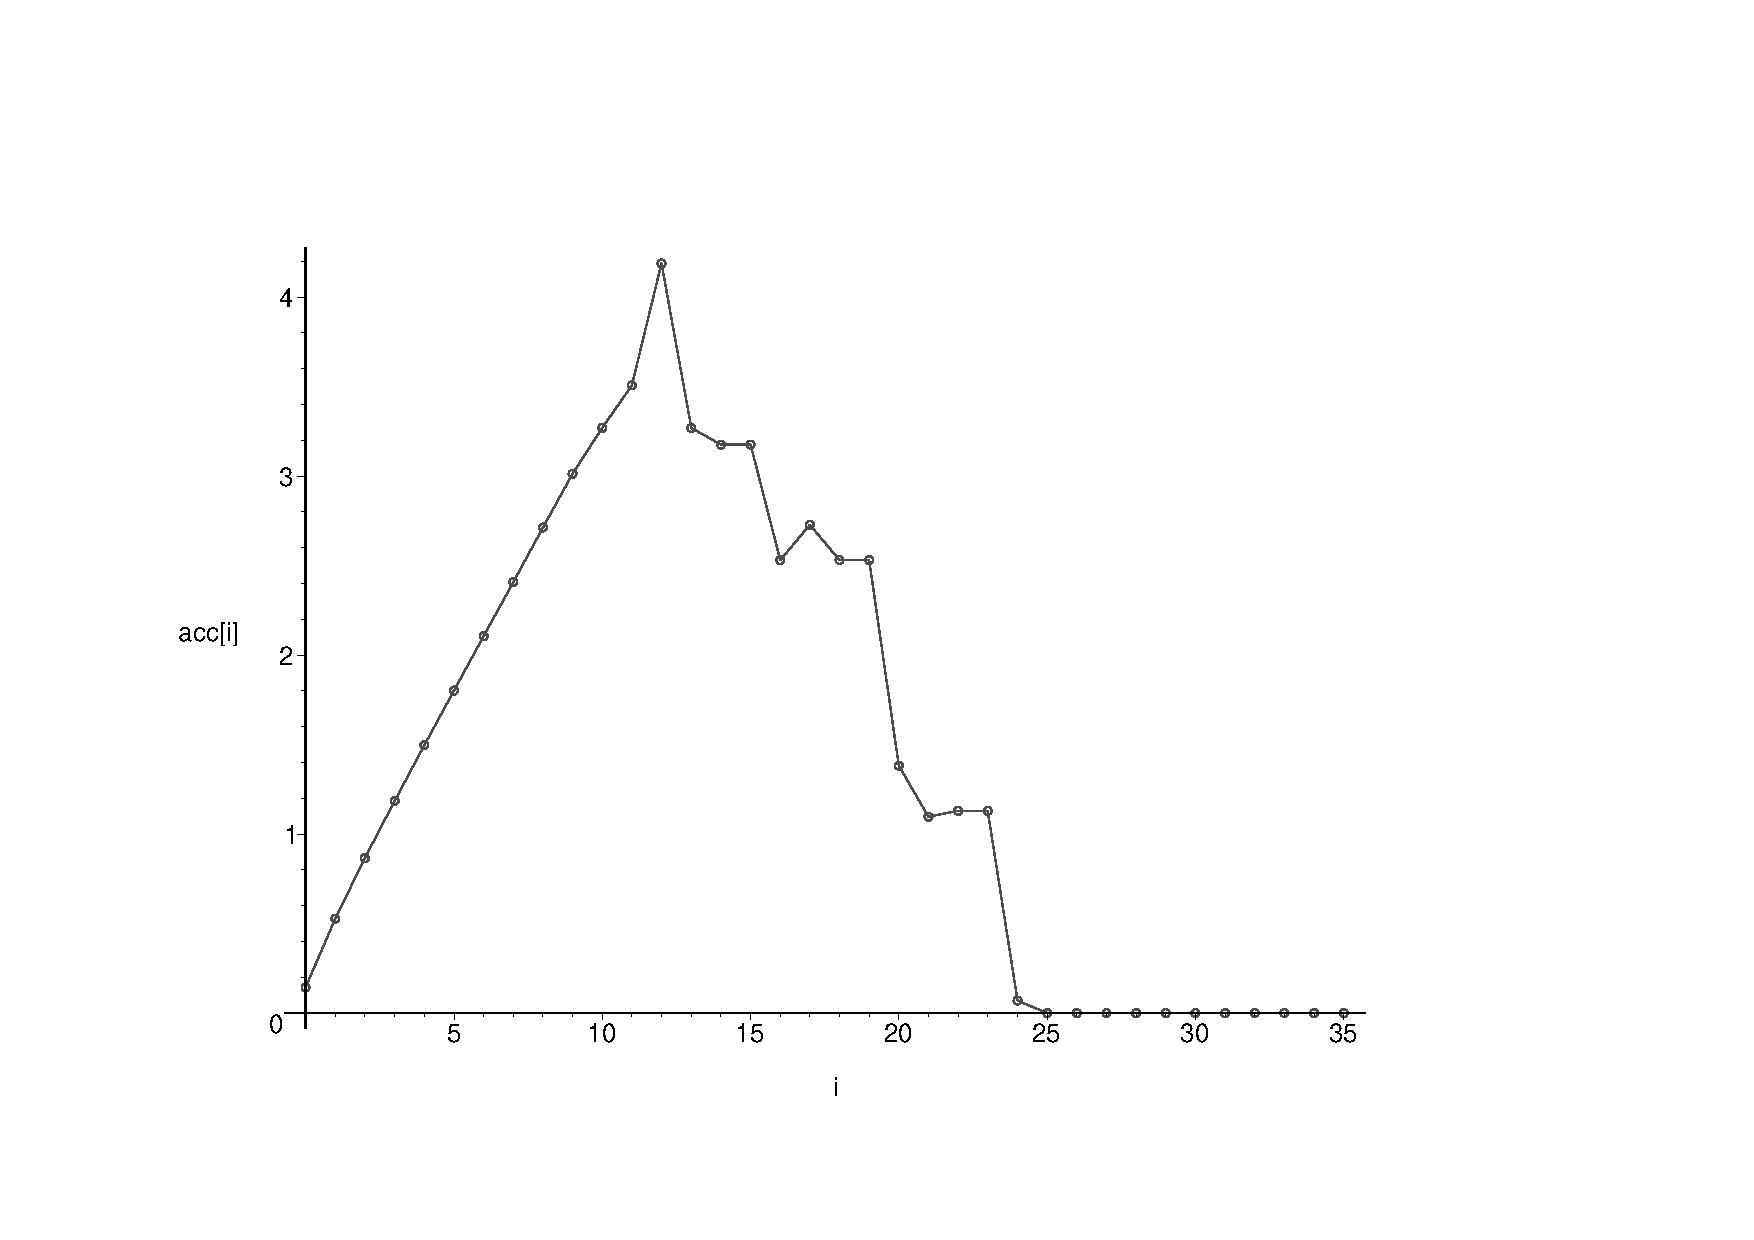
\includegraphics[scale=0.5,angle=0]{wyk1.pdf}
\vspace{-2cm}
\caption{Wielkoœci~\eqref{E:Miara}, typ \texttt{Single}.}\label{W:Wyk1}
\end{figure}
\end{center}

\label{S:Obser}
Jak mo¿na siê by³o spodziewaæ, wyniki poprawiaj¹ siê (uda³o uzyskaæ siê
dok³adnoœæ czterech i oœmiu cyfr dziesiêtnych w arytmetyce pojedynczej 
i podwójnej precyzji, odpowiednio) -- jednak tylko do pewnego momentu. 
Krytycznymi okazuj¹ siê byæ wartoœci $i=12$ (typ \texttt{Single}) oraz $i=26$
(typ \texttt{Double}). Po nich bowiem zaczynamy obserwowaæ utratê dok³adnoœci
obliczeñ. Co jednak najwa¿niejsze, z wykresu odczytaæ mo¿na, ¿e dla $i\geq25$
(typ \texttt{Single}) oraz $i\geq51$ (typ \texttt{Double}) wartoϾ ilorazu
ró¿nicowego wynosi $0$. Zauwa¿amy tutaj rozbie¿noœæ pomiêdzy teori¹ a praktyk¹.
Przecie¿ dla coraz mniejszych wartoœci $h_i$ wyniki powinny byæ coraz
dok³adniejsze. Dlaczego wiêc tak siê nie dzieje? 

\begin{center}
\begin{figure}[!h]
\begin{center}
\vspace{-2cm}
\hspace{0.75cm}
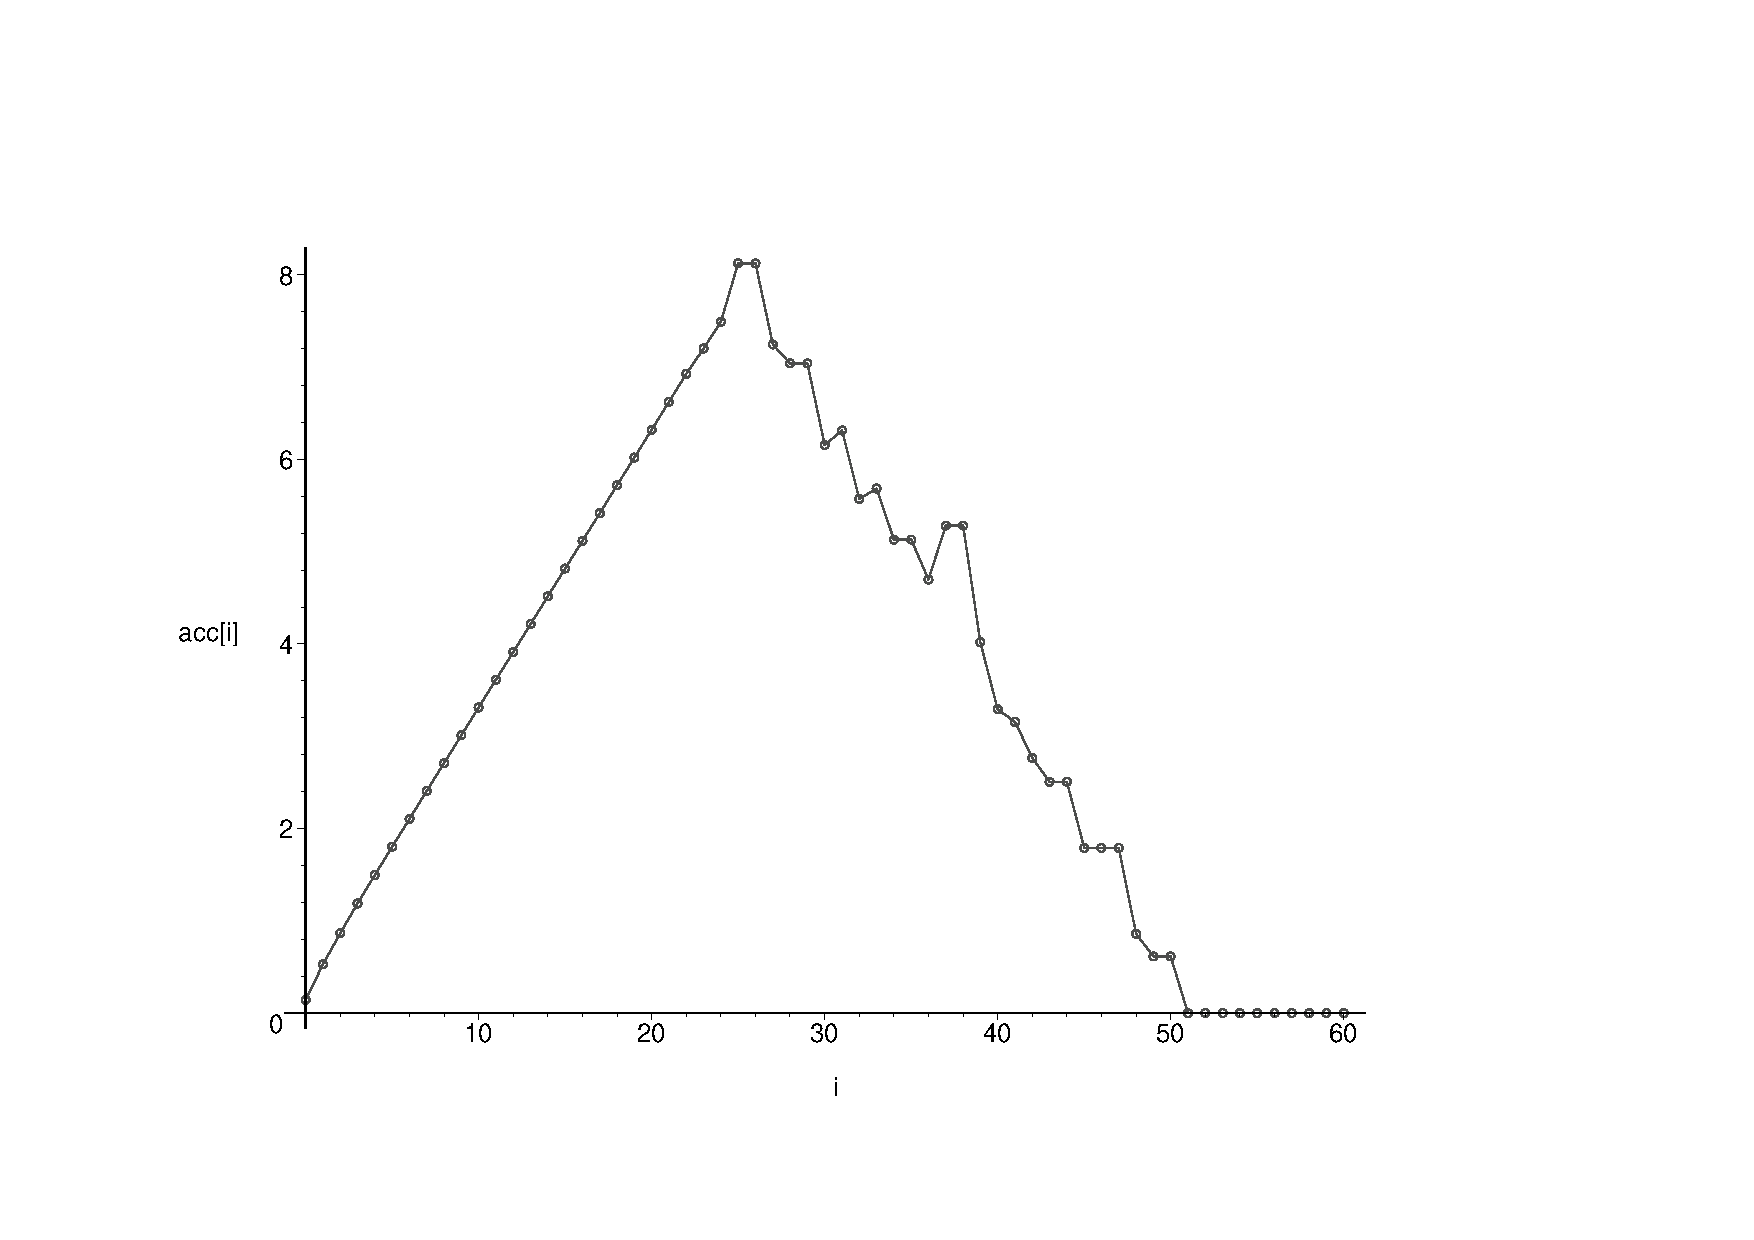
\includegraphics[scale=0.5,angle=0]{wyk2.pdf}
\vspace{-1.5cm}
\caption{Wielkoœci~\eqref{E:Miara}, typ \texttt{Double}.}\label{W:Wyk2}
\end{center}
\end{figure}
\end{center}

Na postawione przed chwil¹ pytanie odpowiedziano w dalszej czêœci tego
paragrafu. Wczeœniej sprawdzono czy opisane zjawisko zale¿y od doboru g³ównych
danych, tj.~fukcji $f$ oraz punktu $x$. W tym celu przeprowadzono testy 
w arytmetyce podwójnej precyzji dla nastêpuj¹cych funkcji:
$$
f_1(x):=e^x,\qquad f_2(x):=\sin\left(\frac{\pi x}{10}\right),\qquad 
f_3(x):=\log{(x+5.1)},
$$
$$
f_4(x):=x^2+x-1,\qquad f_5(x):=\frac{1}{x^2+1},
$$
przybli¿aj¹c wartoœci ich pochodnych, w opisany wy¿ej sposób, w 51
równoodleg³ych punktach przedzia³u $[-5,5]$, tzn.~dla
$$
x_k:=-5+\frac{k}{5}\qquad (k=0,1,\ldots,50),
$$
przy $h_i:=2^{-i}$ $(i=0,1,\ldots,60)$.

We wszystkich testach zaobserwowano to samo zjawisko co poprzednio: na pocz¹tku
ilorazy ró¿nicowe dla rosn¹cych $i$ przybli¿aj¹ coraz lepiej wartoœæ $f'$, a po
przekroczeniu pewnej granicy trac¹ na dok³adnoœci, a¿ w koñcu zawsze otrzymujemy
$0$ dla $i\geq I$ dla pewnego $I\in\mathbb N$.

Wykresy przedstawiaj¹ce wyniki doœwiadczeñ (obliczenia wykonano z podwójn¹
precyzj¹) dla funkcji $f_k$ $(k=1,2,\ldots,5)$ zamieszczono w skrypcie
\texttt{program.mws}. Poniewa¿ charakter wszystkich jest podobny, w sprawozdaniu
ograniczono siê do podania jedynie dwóch, dotycz¹cych funkcji
$f_3(x)=\log(x+5.1)$. 

\begin{center}
\begin{figure}[!h]
\vspace{-3cm}
\hspace{-3cm}
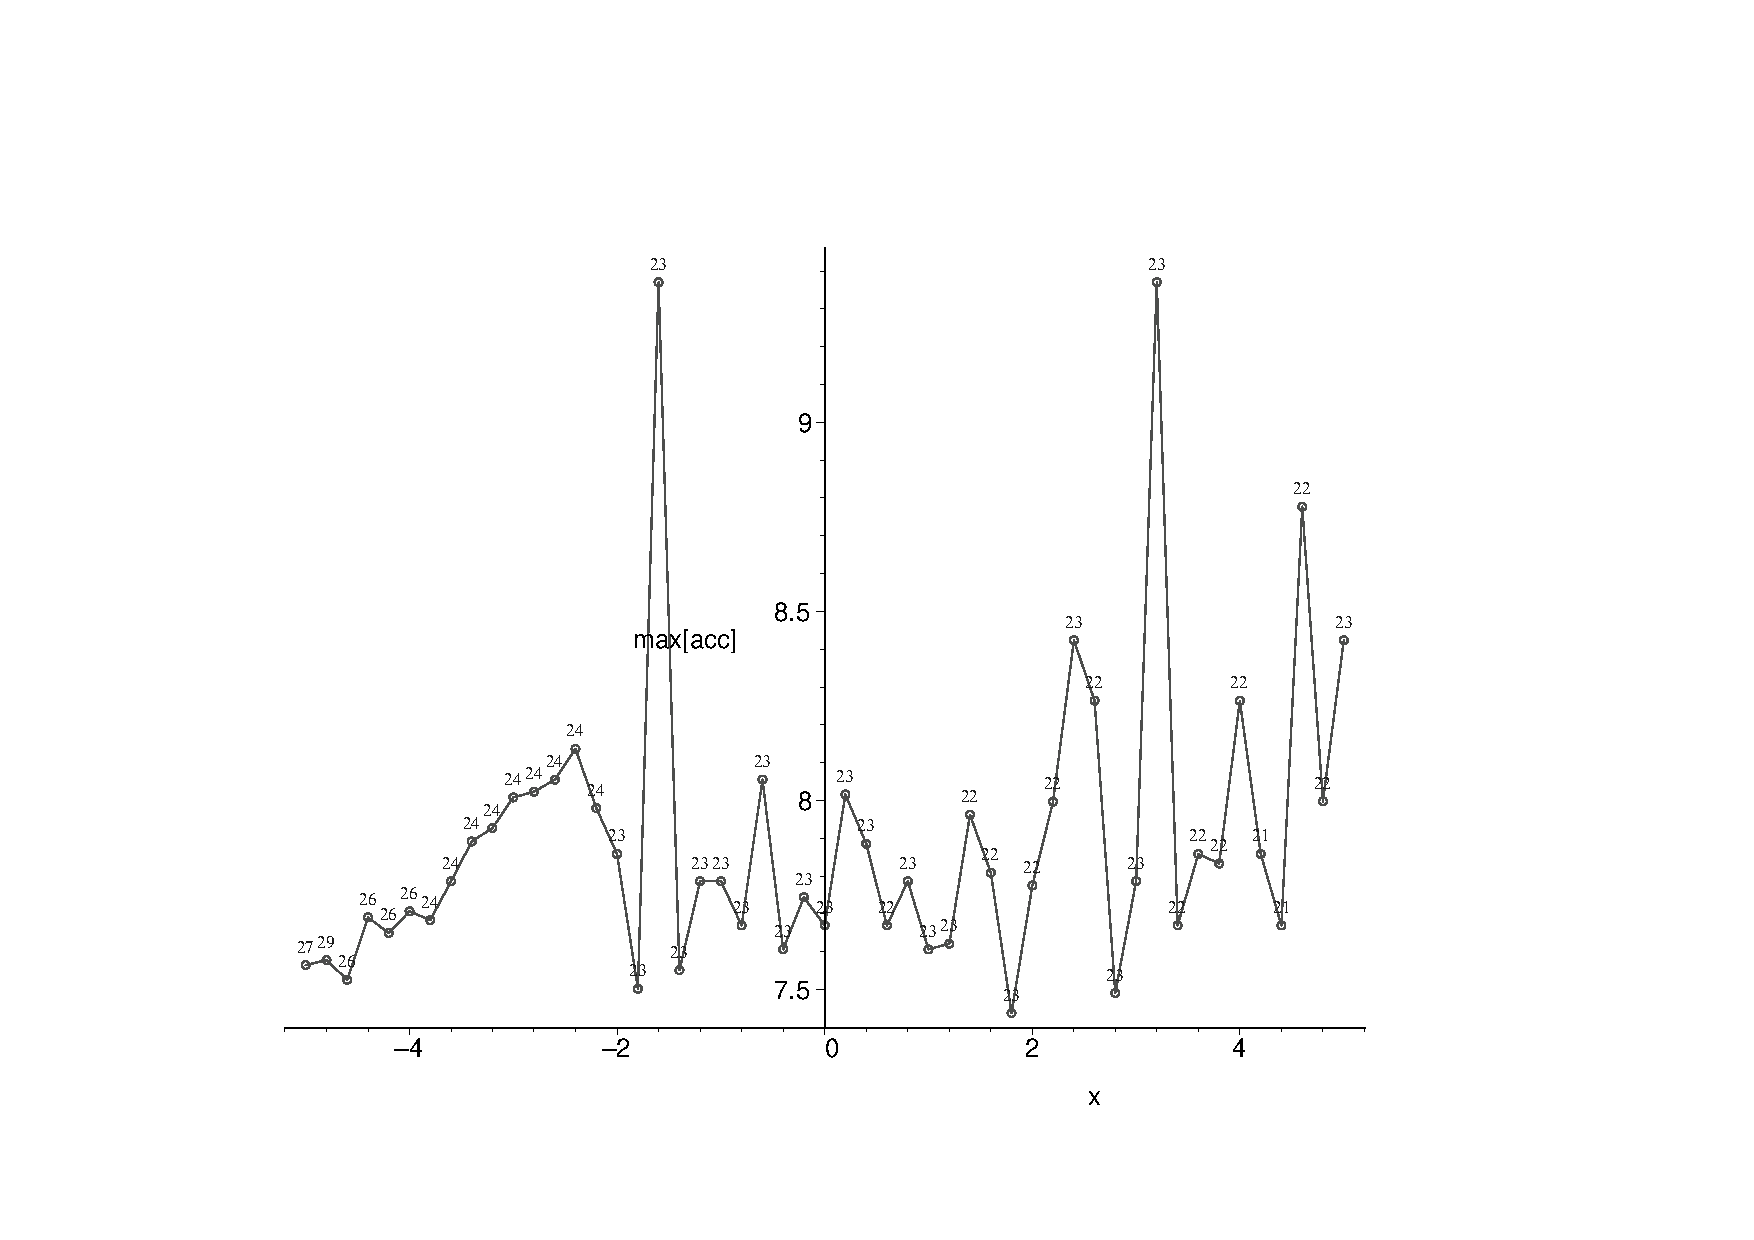
\includegraphics[scale=0.75,angle=0]{wyk3.pdf}
\vspace{-2.25cm}
\caption{Maksymalna dok³adnoœæ przybli¿enia dla $f_3(x)=\log(x+5.1)$, typ
                                              \texttt{Double}.}\label{W:Wyk3}
\end{figure}
\end{center}

I tak, rysunek~\ref{W:Wyk3} przedstawia maksymaln¹ dok³adnoœæ jak¹ uda³o siê
uzyskaæ przybli¿aj¹c $f_3'(x_k)$ $(k=0,1,\ldots,50)$ ilorazem ró¿nicowym
postaci 
$$
\frac{f_3(x_k+h_i)-f(x_k)}{h_i}\qquad (h_i:=2^{-i};\ i=0,1,\ldots,60),
$$
podaj¹c dodatkowo wartoœæ $i$ mu odpowiadaj¹c¹. Z rysunku~\ref{W:Wyk4} odczytaæ
mo¿na natomiast wartoœæ $I$ przy której
$$
\mbox{\textsf{fl}}\left(\frac{f_3(x_k+h_i)-f(x_k)}{h_i}\right)=0
$$
dla $i\geq I$.

Bior¹c pod uwagê wykonane doœwiadczenia, mo¿na stwierdziæ, ¿e poczynione
wczeœniej obserwacje (patrz str.~\ref{S:Obser}) potwierdzaj¹ siê. Jak wiêc
je wyt³umaczyæ? 

\begin{center}
\begin{figure}[!ht]
\vspace{-2cm}
\hspace{-1.5cm}
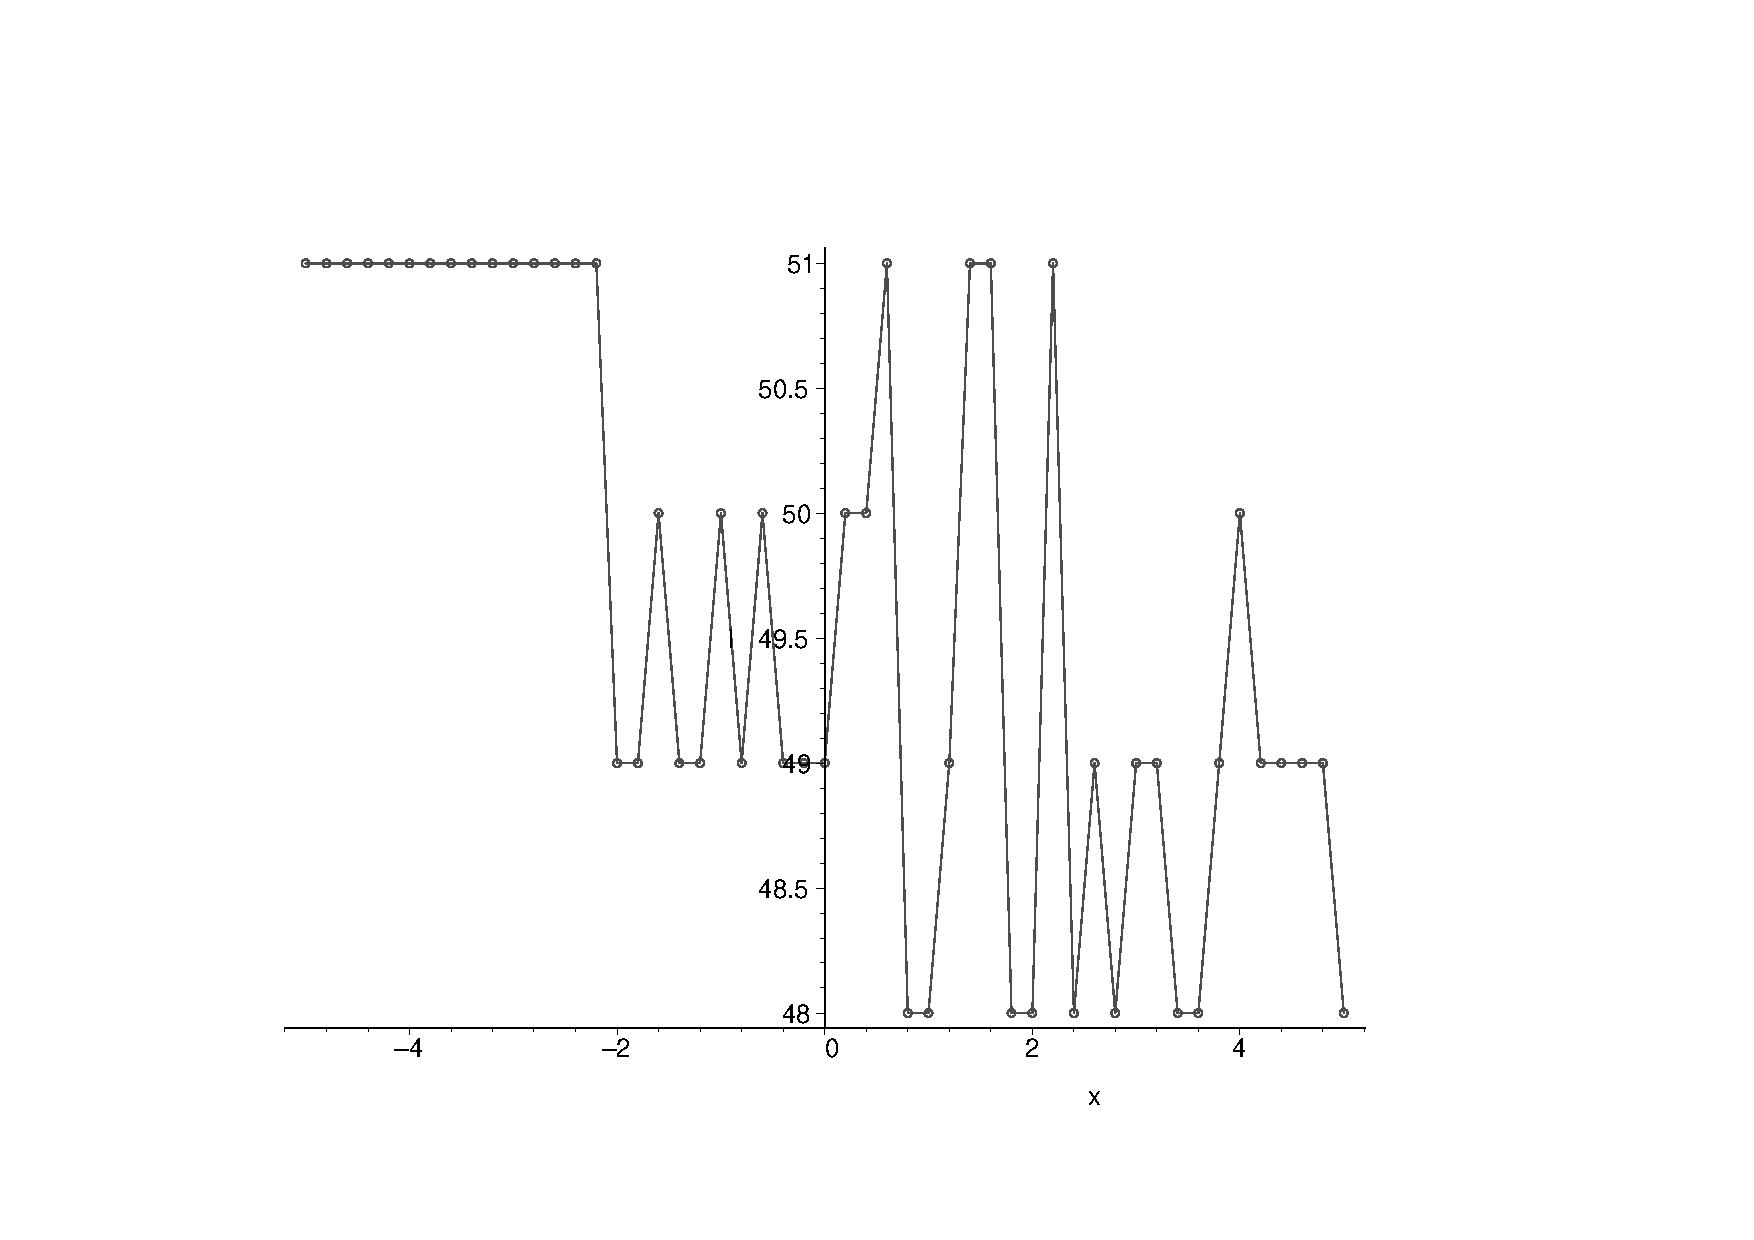
\includegraphics[scale=0.65,angle=0]{wyk4.pdf}
\vspace{-2cm}
\caption{WartoϾ I dla $f_3(x)=\log(x+5.1)$, typ \texttt{Double}.}\label{W:Wyk4}
\end{figure}
\end{center}

Nie jest to trudne. Mo¿na sprawdziæ, np.~eksperymentalnie, albo bior¹c pod uwagê
architekturê komputera, ¿e dla ustalonego  
$a\in X_{\mbox{\textsf{\scriptsize fl}}}$ istnieje w arytmetyce \textsf{fl}
taki zbiór liczb ${\cal A}_{\mbox{\textsf{\scriptsize fl}}}$, ¿e
$$
\mbox{\textsf{fl}}(a+\alpha)=a\qquad (\alpha\in
                                {\cal A}_{\mbox{\textsf{\scriptsize fl}}}).
$$
T³umaczy to fakt, ¿e
$$
\mbox{\textsf{fl}}\left(\frac{f(x_k+h_i)-f(x_k)}{h_i}\right)=0
$$
dla $i\geq I$. Mamy wtedy najczêœciej
$$
\mbox{\textsf{fl}}(f(x_k+h_i))=\mbox{\textsf{fl}}(f(x_k)),
$$
(porównaj z \cite[przyk³ad 1.7]{JJ}). Co wiêcej, w arytmetyce \textsf{fl} nie
mo¿na wykluczyæ sytuacji, w~której implementacja funkcji ró¿nowartoœciowej $f$
(tak¿e bibliotecznej) jest taka, ¿e
$$
\mbox{\textsf{fl}}(f(x_k+h_i))=\mbox{\textsf{fl}}(f(x_k)),
$$
chocia¿ $\mbox{\textsf{fl}}(x_k+h_i)\neq\mbox{\textsf{fl}}(x_k)$. To tak¿e mo¿e
byæ przyczyn¹ zaobserwowanego zjawiska.


%%%%%%%%%%%%%%%%%%%%%%%%%%%%%%%%%%%%%%%%%%%%%%%%%%%%%%%%%%%%%%%%%%%%%%%%%%%%%%%%
%%%%%%%%%%%%%%%%%%%%%%%%%%%%%%%%%%%%%%%%%%%%%%%%%%%%%%%%%%%%%%%%%%%%%%%%%%%%%%%%
\section{Obliczanie pochodnej z du¿¹ dok³adnoœci¹}          \label{S:Obliczanie}
%%%%%%%%%%%%%%%%%%%%%%%%%%%%%%%%%%%%%%%%%%%%%%%%%%%%%%%%%%%%%%%%%%%%%%%%%%%%%%%%
%%%%%%%%%%%%%%%%%%%%%%%%%%%%%%%%%%%%%%%%%%%%%%%%%%%%%%%%%%%%%%%%%%%%%%%%%%%%%%%%
\setcounter{equation}{0}


Z wykonanych eksperymentów jak i z analizy przeprowadzonej w poprzednim
paragrafie wynika, ¿e numeryczne przybli¿anie wartoœci pochodnej $f'(x)$
przy pomocy ilorazu ró¿nicowego \eqref{E:IlorazRoz} nie jest dobrym pomys³em.
W wiêkszoœci testów uda³o siê uzyskaæ dok³adnoœæ równ¹ jedynie mniej wiêcej
po³owie dok³adnoœci z jak¹ wykonywane by³y obliczenia, a wiêc ok.~4--5 cyfr
dziesiêtnych dla typu \texttt{Single} i ok.~7--8 cyfr w wypadku typu
\texttt{Double}. 

Nie jest to rezultat satysfakcjonuj¹cy. Ale czy mog³o byæ inaczej? Stosuj¹c
wzór Taylora, ³atwo uzasadniæ, ¿e
$$
f'(x)=\frac{f(x+h)-f(x)}{h}+{\cal O}(h).
$$
Tak wiêc, przybli¿enie $f'(x)$ ilorazem ró¿nicowym~\eqref{E:IlorazRoz} obarczone
jest b³êdem proporcjonalnym do $h$. Dodaj¹c do tego specyfikê arytmetyki
\textsf{fl}, jasne ju¿ staje siê dlaczego podejœcie takie nie jest w³aœciwe.

Jak zatem wyznaczyæ numerycznie pochodn¹ z wiêksz¹ dok³adnoœci¹? Mo¿na stosowaæ
np.~metody zwi¹zane z interpolacja czy aproksymacj¹, albo jeszcze bardziej
wyrafinowane podejœcia. Jak siê jednak okazuje istniej¹ prostsze, a równie
skuteczne, metody bazuj¹ce jedynie na wzorze Taylora. W paragrafie tym
krótko je opisano.

Stosuj¹c technikê omówion¹ na jednym z repetytoriów z analizy numerycznej, 
tj.~wykorzystuj¹c odpowiednie rozwiniêcia w szereg Taylora, a nastêpnie
rozwi¹zuj¹c pewne uk³ady równañ liniowych, mo¿na wyprowadziæ nastêpuj¹ce wzory
(szczegó³owe obliczenia pominiêto):
\begin{eqnarray*}
&&f'(x)=\frac{f(x+h)-f(x-h)}{2h}+{\cal O}(h^2),\\[1ex]
&&f'(x)=\frac{f(x-2h)-8f(x-h)+8f(x+h)-f(x+2h)}{12h}+{\cal O}(h^4),\\[1ex]
&&f'(x)=\frac{1}{60h}\Big(f(x+3h)-9f(x+2h)+45f(x+h)-\\
&&\phantom{f'(x)=\frac{1}{60h}\Big(f(x+3h)-9f(x+2h)}
                          -45f(x-h)+9f(x-2h)-f(x-3h)\Big)+{\cal O}(h^6).							      
\end{eqnarray*}

Podane wy¿ej wyra¿enia lepiej przybli¿aj¹ wartoœæ $f'(x)$. Ich b³¹d jest
proporcjonalny do $h^2$, $h^4$ i $h^6$, odpowiednio. Co prawda, aby je wyznaczyæ
nale¿y obliczyæ wartoœæ funkcji $f$ w~wiêkszej liczbie punktów, ale -- jak
wynika z przeprowadzonych doœwiadczeñ (patrz do³¹czony do sprawozdania skrypt
\texttt{program.mws}) i podanych ni¿ej wykresów -- warto ponieœæ dodatkowy
koszt, aby uzyskaæ wiêksz¹ dok³adnoœæ.

Poni¿ej omówiono pokrótce tylko jeden z przeprowadzonych eksperymentów. Niech
bêdzie
$$
f_2(x)=\sin\left(\frac{\pi x}{10}\right)
$$
oraz $x_k:=-5+\frac{k}{5}$ $(k=0,1,\ldots,50)$. Do numerycznego przybli¿enia
wartoœci pochodnej w~punktach $x_k$, tzn. 
$$
f_2'(x_k)=\frac{\pi}{10}\cos\left(\frac{\pi x_k}{10}\right)\qquad
                                                            (k=0,1,\ldots,50),
$$
u¿yto nastêpuj¹cego wzoru: 
$$
df_{2,k}^{[6]}:=\frac{f_2(x+3h)-9f_2(x+2h)+45f_2(x+h)-
                                       45f_2(x-h)+9_2f(x-2h)-f_2(x-3h)}{60h},
$$
przyjmuj¹c $\displaystyle h:=2^{-7}$ i wykonuj¹c obliczenia w typie podwójnej
precyzji.

Rysunkek~\ref{W:Wyk5} przedstawia wielkoœci
\begin{equation}\label{E:Miara2}
\texttt{acc[6,k]}:=
\left\{
\begin{array}{ll}
-\log_{10}\left|df_{2,k}^{[6]}\right| & \mbox{dla $k=0$ i $k=50$},\\[2ex]
\displaystyle 
-\log_{10}\left|1-\frac{df_{2,k}^{[6]}}{f_2'(x_k)}\right| & 
                                                 \mbox{dla $k=1,2,\ldots,49$}
\end{array}
\right.
\end{equation}
(porównaj z~\eqref{E:Miara}). Mo¿na z niego odczytaæ, ¿e otrzymane wyniki s¹
lepsze. Uda³o siê uzyskaæ dok³adnoœæ ok.~12--14 cyfr dziesiêtnych.

\begin{center}
\begin{figure}[!ht]
\vspace{-2cm}
\hspace{-1.5cm}
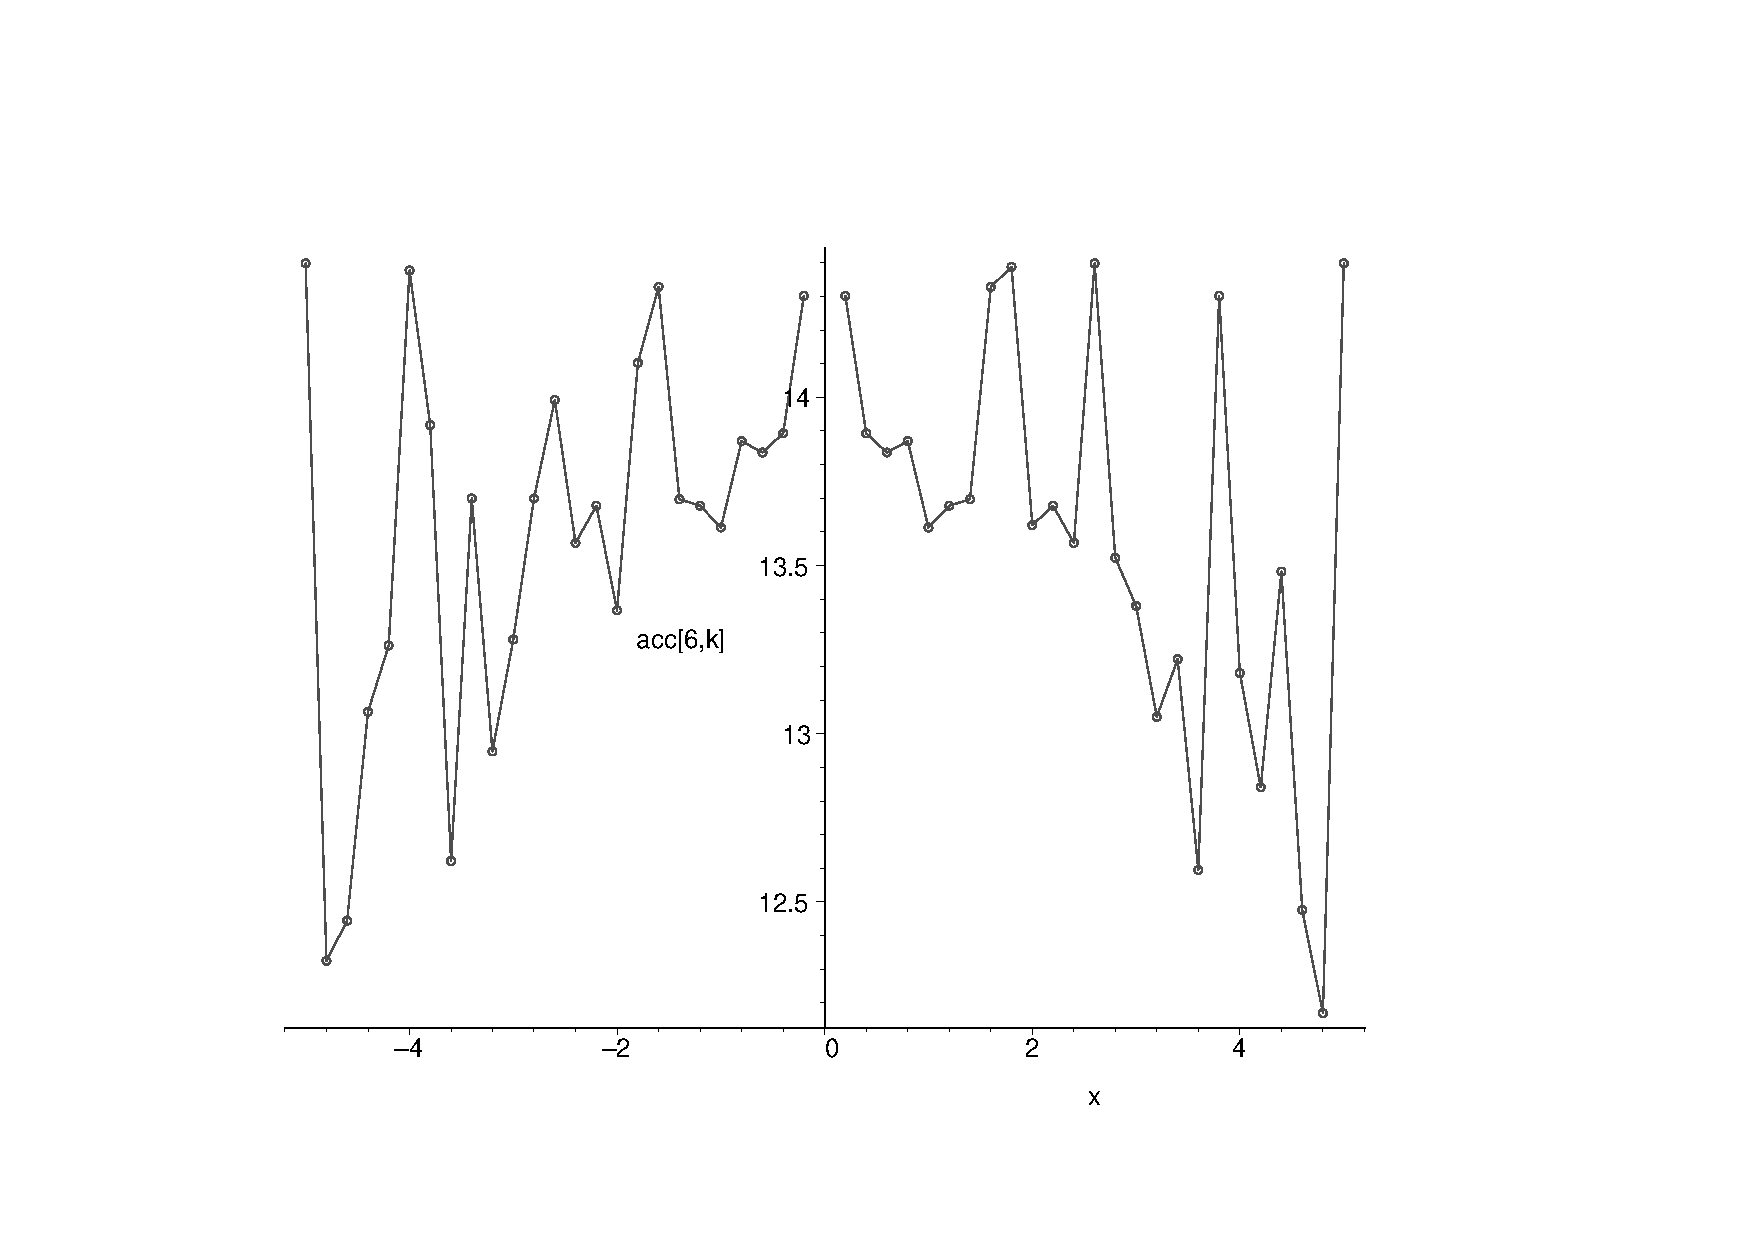
\includegraphics[scale=0.65,angle=0]{wyk5.pdf}
\vspace{-2cm}
\caption{Wielkoœci~\eqref{E:Miara2}, typ \texttt{Double}.}\label{W:Wyk5}
\end{figure}
\end{center}


%%%%%%%%%%%%%%%%%%%%%%%%%%%%%%%%%%%%%%%%%%%%%%%%%%%%%%%%%%%%%%%%%%%%%%%%%%%%%%%
%%%%%%%%%%%%%%%%%%%%%%%%%%%%%%%%%%%%%%%%%%%%%%%%%%%%%%%%%%%%%%%%%%%%%%%%%%%%%%%%
%% Bibliografia
%%%%%%%%%%%%%%%%%%%%%%%%%%%%%%%%%%%%%%%%%%%%%%%%%%%%%%%%%%%%%%%%%%%%%%%%%%%%%%%
%%%%%%%%%%%%%%%%%%%%%%%%%%%%%%%%%%%%%%%%%%%%%%%%%%%%%%%%%%%%%%%%%%%%%%%%%%%%%%%%
%\newpage
\thispagestyle{empty}
\begin{thebibliography}{99}

\bibitem{BD}  A.~Bj\"orck, G.~Dahlquist, \textit{Metody numeryczne\/}, PWN,
              1987.

\bibitem{ChK} W.~Cheney, D.~Kincaid, \textit{Analiza numeryczna\/}, WNT, 2006.

\bibitem{JJ}  J.~i~M.~Jankowscy, \textit{Przegl¹d metod i algorytmów
              numerycznych\/}, cz. 1, WNT, 1988.

\bibitem{L}   S.~Lewanowicz, \textit{Notatki do wyk³adu z analizy numerycznej},
              Wroc³aw, 2011.
	  
\end{thebibliography}

\end{document}

